\textbf{Ejemplo 7}\\
Un fabricante o proveedor de bicicletas recibe un pedido de compra de 50 unidades para un almacén por valor de 5 millones COP, pero el almacén pide un plazo de 90 días para pagar. El fabricante o proveedor acepta el pedido, pero solicita que una entidad financiera garantice el pago futuro, por tal motivo el dueño del almacén se dirige a su banco y le solicita que expida una aceptación bancaria por 5 millones COP con vencimiento en 90 días. El banco le entrega al almacén la aceptación y este se la entrega al fabricante o proveedor. Este último puede guardar la aceptación y cobrarla al banco a su vencimiento o puede negociarla en el mercado secundario. Si el fabricante necesita el dinero deberá vender la aceptación, la podrá vender en el mercado no bursátil, donde no pagará a comisionistas de bolsa, o al mercado bursátil (bolsa de valores) a través de un comisionista de bolsa que cobra una comisión por sus servicios. Cuando la fecha de la aceptación se termine, el dueño del almacén deberá pagar al banco. El banco deberá pagar la aceptación al tenedor de la aceptación, así sea que el almacén pague al banco o no.

Calcular el precio de venta (en porcentaje) y el valor de venta de la aceptación, en el mercado fuera de bolsa y en la bolsa cediendo una rentabilidad del 30\% periodo año vencido (tasa de registro bursátil). Para el caso bursátil, el comisionista vendedor cobra una comisión del 0,5\% periodo año vencido. Tomar el año de 365 días. Calcular los valores faltando los siguientes días al vencimiento:

Calcular:
a) 90 días al vencimiento\\
b) 40 días al vencimiento\\
c) 10 días al vencimiento

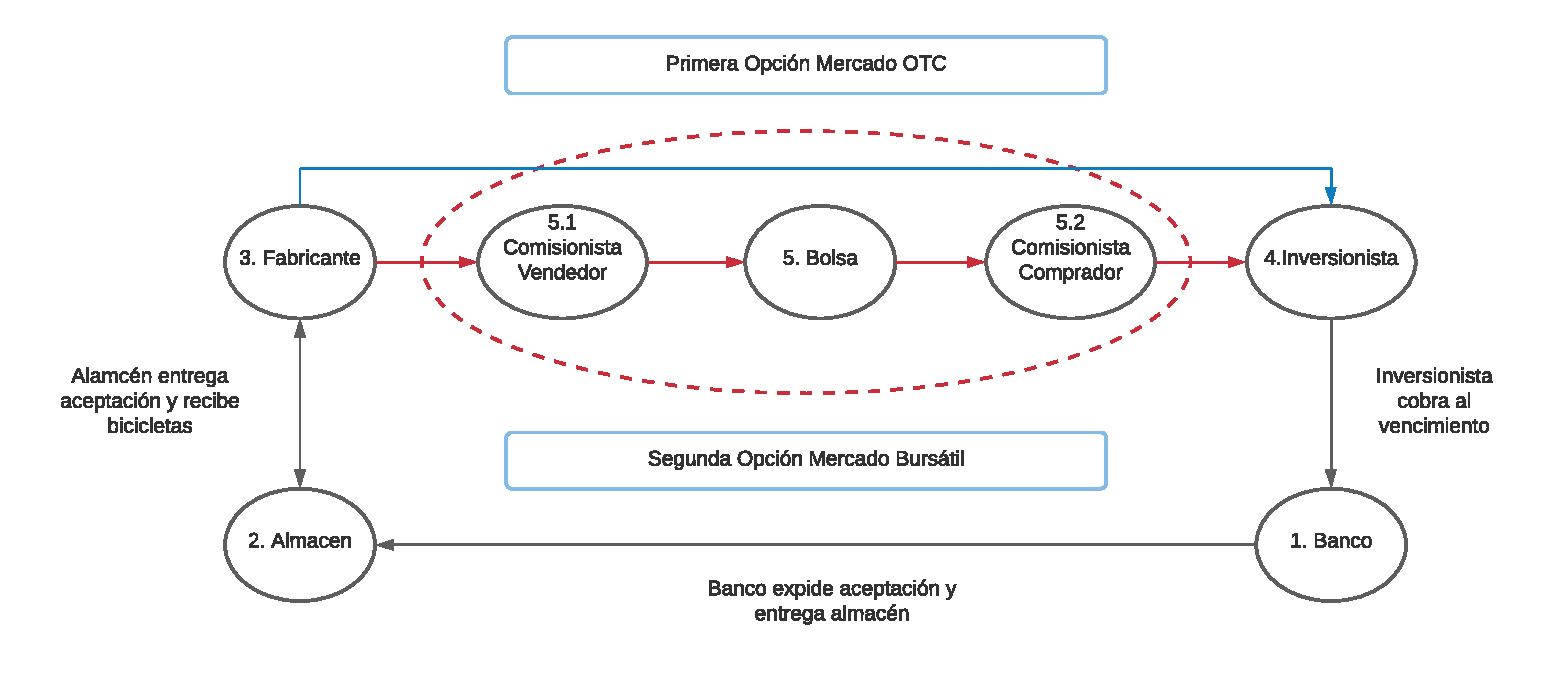
\includegraphics[scale=0.55, width=16.4cm, height=10.5cm]{7/Capitulo3Ejercicio7.pdf}\newline
\newpage %USAR SOLO SI EL SOLUCIÓN QUEDA SOLO Y ES NECESARIO BAJARLO A LA SIGUIENTE PAG

\textbf{Solución.}

\begin{center}
	\textbf{Primera opción (Mercado extra bursátil)}
\end{center}

a) Para 90 días antes del vencimiento:
\begin{center}
	\renewcommand{\arraystretch}{1.5}% Margenes de las celdas
	\begin{longtable}[H]{|p{0.33\linewidth}|p{0.33\linewidth}|p{0.33\linewidth}|}
		\hline
		\rowcolor[HTML]{FFB183}
		\multicolumn{3}{|c|}{\cellcolor[HTML]{FFB183}\textbf{1. Asignación período focal}} \\ \hline
		\multicolumn{3}{|c|}{$pf : \frac{90}{365} = 0.246 \textit{ pav}$} \\ \hline
		\rowcolor[HTML]{FFB183}
		\multicolumn{3}{|c|}{\cellcolor[HTML]{FFB183}\textbf{2. Declaración de variables}} \\ \hline
		\multicolumn{1}{|c|}{\cellcolor[HTML]{FFB183}\textbf{Valores monetarios}} & 
		\multicolumn{1}{|c|}{\cellcolor[HTML]{FFB183}\textbf{Valores no monetarios}} &
		\multicolumn{1}{|c|}{\cellcolor[HTML]{FFB183}\textbf{Incógnitas}} \\ \hline
		$F = 5{.}000{.}000\ COP$ & $i = 30\%\textit{ pav}$ & $P_{v} = \ ? \% $ \\
		$Comisión = 0.5\% \textit{ pav}$ & $n = \frac{90}{365} = 0.246\ pav $ & $V_{v} =\ ?\ COP$ \\ \hline
		\rowcolor[HTML]{FFB183}
		\multicolumn{3}{|c|}{\cellcolor[HTML]{FFB183}\textbf{3. Diagrama de flujo de caja}} \\ \hline
		\multicolumn{3}{|c|}{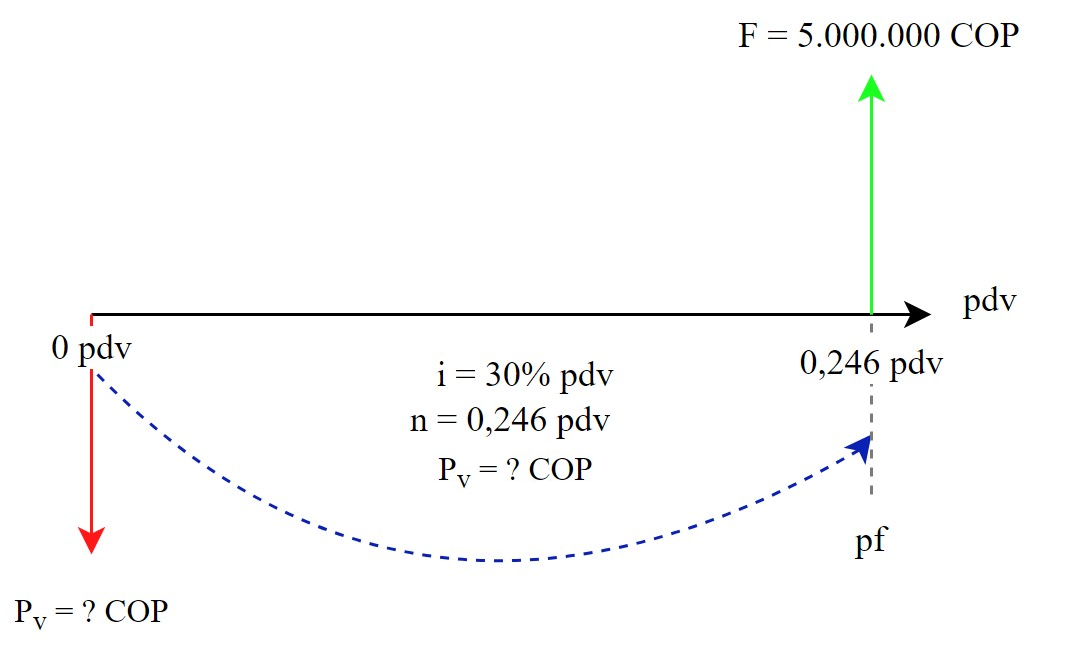
\includegraphics[trim=-5 -5 -5 -5, width=16.4cm, height=10.5cm]{3_Capitulo/img/ejemplos/7/7.1.a.png}} \\ \hline
		\rowcolor[HTML]{FFB183}
		\multicolumn{3}{|c|}{\cellcolor[HTML]{FFB183}\textbf{4. Declaración de fórmulas}} \\ \hline
		\multicolumn{3}{|c|}{$F = P(1 + i)^n$ \hspace{2mm} Valor futuro} \\ \hline
		\rowcolor[HTML]{FFB183}
		\multicolumn{3}{|c|}{\cellcolor[HTML]{FFB183}\textbf{5. Desarrollo matemático}} \\ \hline
		\multicolumn{3}{|C{\linewidth}|}{
			\newline
			\vspace{4mm}
			Para el mercado extrabursátil (fuera de bolsa)
			\vspace{1mm}
			$V_{veb} = (5{.}000{.}000 \ COP) (1 + 0.3)^\frac{-90}{365} = 4{.}854{.}623.29\ COP \textit{ Ecuación de equivalencia}$
			
			$P_{veb} = \frac{4{.}854{.}623.29}{5{.}000{.}000} = 0.9709$
		} \\ \hline
		\rowcolor[HTML]{FFB183}
		\multicolumn{3}{|c|}{\cellcolor[HTML]{FFB183}\textbf{6. Respuesta}} \\ \hline
		\multicolumn{3}{|C{\textwidth}|}{
			$V_{veb} = 4{.}854{.}623.29\ COP$
            
			$P_{veb} \equiv 97.09 \textit{ COP}\%$
		} \\ \hline
	\end{longtable}
\end{center}